\documentclass[12pt, a4paper, oneside]{ctexart}
\usepackage{amsmath, amsthm, amssymb, appendix, bm, graphicx, mathrsfs, geometry, xcolor,
 subcaption, float, fancyhdr}
\geometry{left=2.54cm, right=2.54cm, top=3.18cm, bottom=3.18cm}
\usepackage[colorlinks, linkcolor=black]{hyperref}
\usepackage{multirow}
\usepackage{listings}		% 为了避免与页眉的兼容问题可将listings放入table环境中
\lstset{
    basicstyle          =   \sffamily,          % 基本代码风格
    keywordstyle        =   \color{blue},          % 关键字风格
    keywordstyle    =   [2] \color{teal},
    commentstyle        =   \rmfamily\itshape,  % 注释的风格,斜体
    stringstyle         =   \ttfamily,  % 字符串风格
    flexiblecolumns,                % 别问为什么,加上这个
    numbers             =   left,   % 行号的位置在左边
    showspaces          =   false,  % 是否显示空格,显示了有点乱,所以不现实了
    numberstyle         =   \zihao{-5}\ttfamily,    % 行号的样式,小五号,tt等宽字体
    showstringspaces    =   false,
    captionpos          =   t,      % 这段代码的名字所呈现的位置,t指的是top上面
    frame               =   lrtb,   % 显示边框
    basicstyle          =   \zihao{-4}\ttfamily,
    stringstyle         =   \color{magenta},
    commentstyle        =   \color{red}\ttfamily,
    breaklines          =   true,   % 自动换行,建议不要写太长的行
    columns             =   fixed,  % 如果不加这一句,字间距就不固定,很丑,必须加
    basewidth           =   0.5em,
}
\pagestyle{fancy}
\lhead{\textit{\leftmark}}
\chead{} 
\rhead{\textit{\rightmark}}
\lfoot{} 
\cfoot{\thepage}
\rfoot{}
\renewcommand\headrulewidth {0pt} 

\linespread{1.5}
\renewcommand{\abstractname}{\Large\textbf{摘要}}

\begin{document}

\thispagestyle{empty}

\begin{figure}[t]
    \centering
    
\includegraphics[width=13cm]{../pic/xjtu.png}
\end{figure}

\vspace*{\fill}
    \begin{center}
        \centering
        \vspace{-3cm}
        \fangsong\huge{本科生课程报告} \\\kaishu \Huge{\textbf{基于数据流图的高校学生管理系统\\的UML系列图建模}}
    \end{center}
\vspace*{\fill}

\begin{table}[b]
    \centering
    \large
    \begin{tabular}{ll}
        \textbf{课程:} & 软件系统设计与分析 \\
        \textbf{姓名:} & 杨豪 \\
        \textbf{班级:} & 软件2101 \\
        \textbf{时间:} & 2022年11月 \\
    \end{tabular}
\end{table}

\newpage

\thispagestyle{empty}
\begin{abstract}
    UML(Unified Modeling Language,统一建模语言)是用来对软件密集系统进行可视化建模的一种语言。UML的定义包括UML语义和UML表示法两个元素。
    UML包括一系列图表,在构建和分析大型复杂软件系统时体现出极高的效率。本文采用PowerDesigner从一个已有数据流图的高校学生管理系统开始,展示了逐步从
    功能模型(USE CASE图,并简要描述事件流)、动态模型(活动图与分析时序图)、静态模型(分析类图)以及数据库ER模型建立出完整的模型。
    \par\textbf{关键词:}UML建模; 数据流图; 学生管理系统; 系统分析与设计.
\end{abstract}

\newpage
\pagenumbering{Roman}
\setcounter{page}{1}
\thispagestyle{plain}
\tableofcontents
\newpage
\setcounter{page}{1}
\pagenumbering{arabic}

\section{数据流图}

\begin{figure}[H]
    \centering
    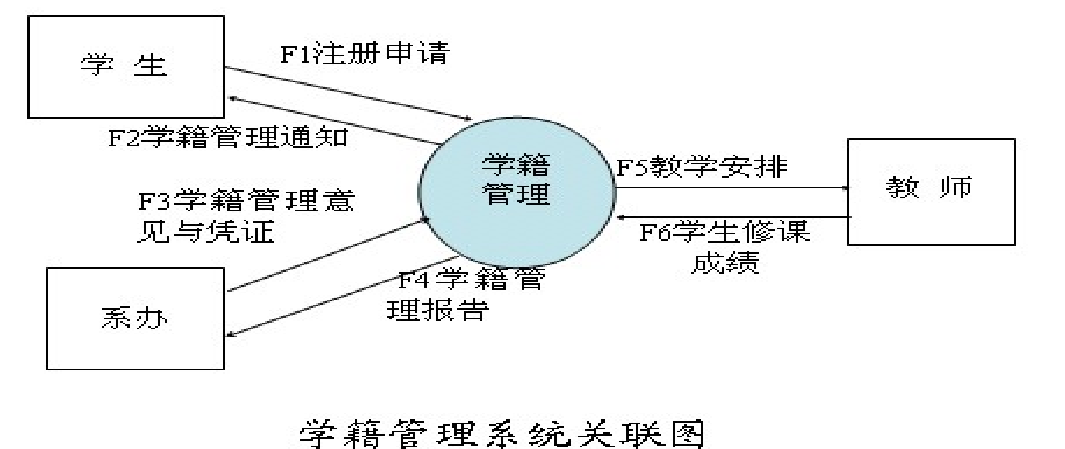
\includegraphics[width = 1\textwidth]{../pic/1/1.1.png}
\end{figure}

\begin{figure}[H]
    \centering
    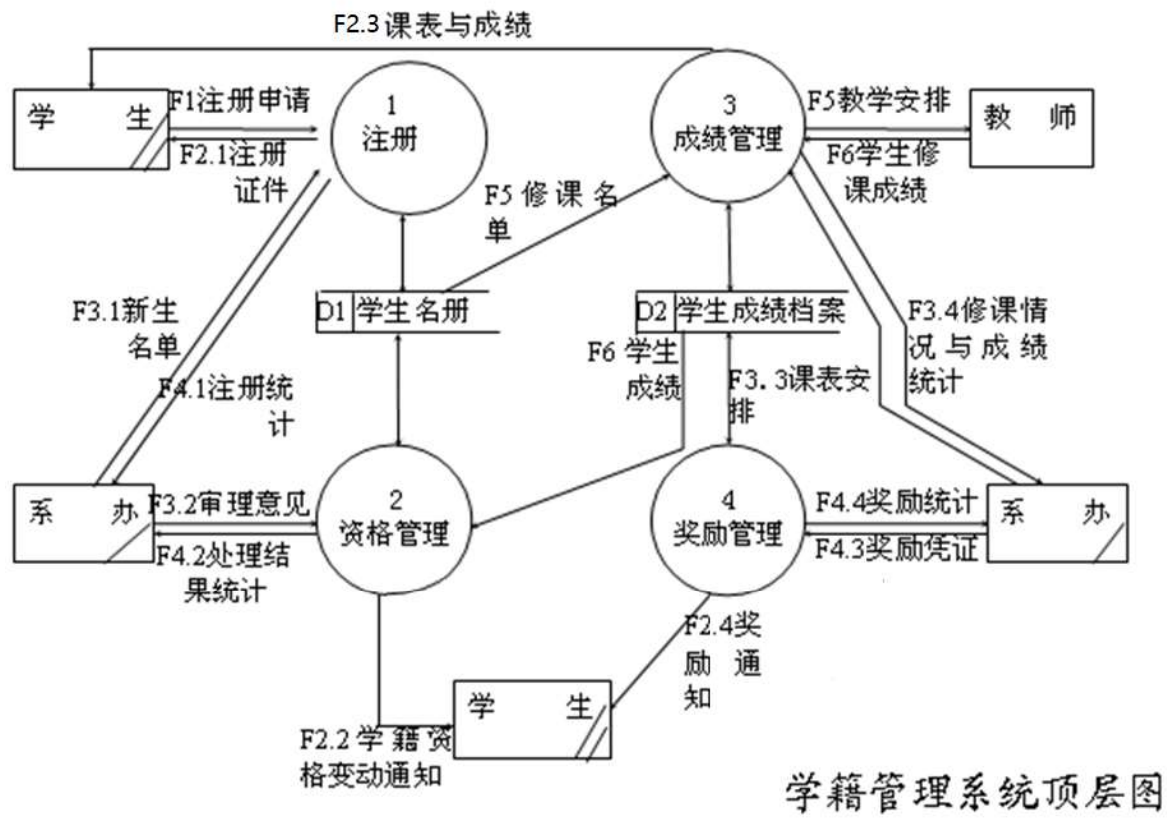
\includegraphics[width = 1\textwidth]{../pic/1/1.2.png}
\end{figure}

\section{功能模型}

\subsection{USE CASE图}

分析两层数据流图可得用例图如下

\begin{figure}[H]
    \centering
    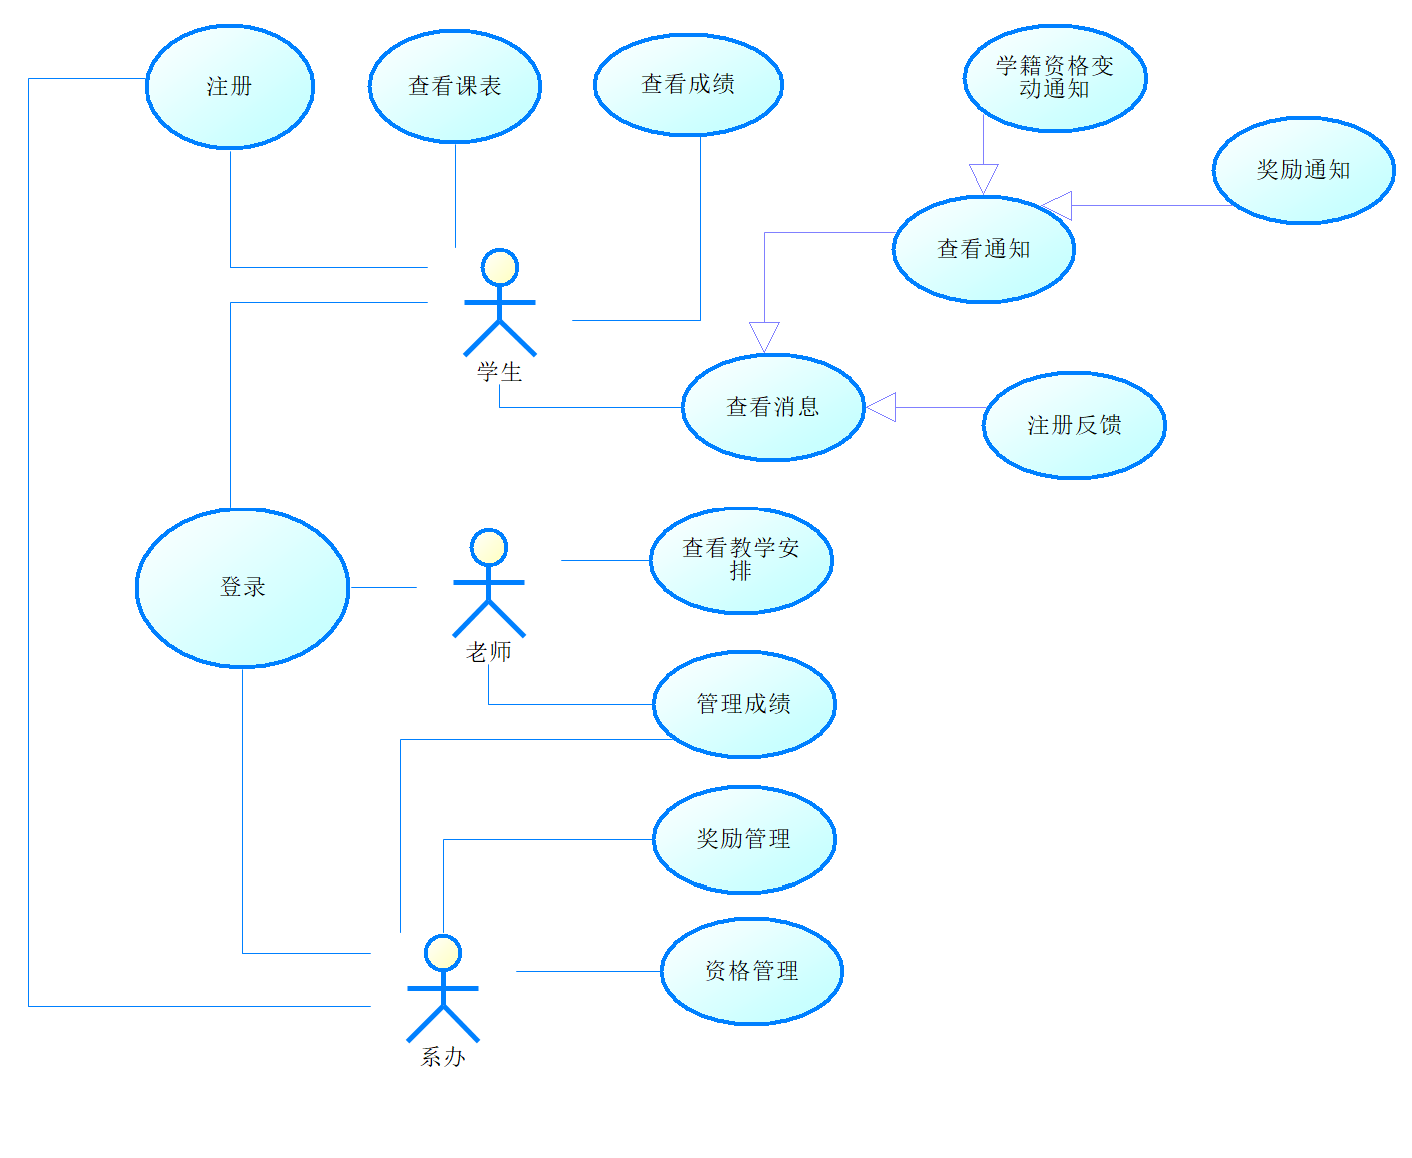
\includegraphics[width = 1\textwidth]{../pic/2.png}
\end{figure}

\subsection{用例描述}

选取涉及参与者最多的五个用例:登录、注册、资格管理、成绩管理、奖励管理作出用例描述表

\begin{table}[H]
    \centering
    \begin{tabular}{|c|cc|}
        \hline
        用例名称                   & \multicolumn{2}{c|}{登录}                       \\ \hline
        用例参与者                  & \multicolumn{2}{c|}{学生、系办、教师}                 \\ \hline
        概述                     & \multicolumn{2}{c|}{用户登录进入系统}                 \\ \hline
        前置条件                   & \multicolumn{2}{c|}{系统运行正常}                   \\ \hline
        后置条件                   & \multicolumn{2}{c|}{用户(参与者)发起各种操作}            \\ \hline
        \multirow{3}{*}{基本事件流} & \multicolumn{1}{c|}{1}  & 参与者输入用户名和密码         \\ \cline{2-3} 
                            & \multicolumn{1}{c|}{2}  & 系统确认用户名密码无误         \\ \cline{2-3} 
                            & \multicolumn{1}{c|}{3}  & 系统展示对应于参与者权限的登陆界面   \\ \hline
        \multirow{3}{*}{扩展事件流} & \multicolumn{1}{c|}{1a} & 若用户名或密码不合法,系统提示对应消息 \\ \cline{2-3} 
                            & \multicolumn{1}{c|}{2a} & 若用户名不存在,系统提示对应消息    \\ \cline{2-3} 
                            & \multicolumn{1}{c|}{2b} & 若用户名和密码不符,系统提示对应消息  \\ \hline
    \end{tabular}
    \caption{登录用例描述表}
\end{table}

\begin{table}[H]
    \centering
    \begin{tabular}{|c|cc|}
        \hline
        用例名称                   & \multicolumn{2}{c|}{注册}                                  \\ \hline
        用例参与者                  & \multicolumn{2}{c|}{学生、系办}                               \\ \hline
        概述                     & \multicolumn{2}{c|}{系办发布新生名单,学生申请注册}                     \\ \hline
        前置条件                   & \multicolumn{2}{c|}{学生成功确认身份并登陆系统}                       \\ \hline
        后置条件                   & \multicolumn{2}{c|}{注册完成,得到注册统计数据}                       \\ \hline
        \multirow{4}{*}{基本事件流} & \multicolumn{1}{c|}{1}  & 系办向系统发布注册名单                    \\ \cline{2-3} 
                            & \multicolumn{1}{c|}{2}  & 学生发起注册申请                       \\ \cline{2-3} 
                            & \multicolumn{1}{c|}{3}  & 系统向学生发送注册证件                    \\ \cline{2-3} 
                            & \multicolumn{1}{c|}{4}  & 系统发起注册统计                    \\ \hline
        \multirow{2}{*}{扩展事件流} & \multicolumn{1}{c|}{2a} & 系统中若未发现该学生则提示“找不到您的信息,请联系系办确认” \\ \hline
                            & \multicolumn{1}{c|}{3a} & 注册人满后再进入第4步,否则到截止时间再发统计        \\ \hline
    \end{tabular}
    \caption{注册用例描述表}
\end{table}

\begin{table}[H]
    \centering
    \begin{tabular}{|c|cc|}
    \hline
    用例名称                   & \multicolumn{2}{c|}{资格管理}                  \\ \hline
    用例参与者                  & \multicolumn{2}{c|}{系办、学生(次要)}             \\ \hline
    概述                     & \multicolumn{2}{c|}{系办审查学生的资格}             \\ \hline
    前置条件                   & \multicolumn{2}{c|}{学生、系办成功登陆系统,系统得到学生成绩}  \\ \hline
    后置条件                   & \multicolumn{2}{c|}{完成资格管理,得到处理结果统计}       \\ \hline
    \multirow{5}{*}{基本事件流} & \multicolumn{1}{c|}{1}  & 系办点击资格管理         \\ \cline{2-3} 
                           & \multicolumn{1}{c|}{2}  & 系统展示待审查的条目       \\ \cline{2-3} 
                           & \multicolumn{1}{c|}{3}  & 系办给出审理意见         \\ \cline{2-3} 
                           & \multicolumn{1}{c|}{4}  &  系统向学生发送学籍资格变动通知       \\ \cline{2-3} 
                           & \multicolumn{1}{c|}{5}  &  系统生成处理结果统计 \\ \hline
    \multirow{2}{*}{扩展事件流} & \multicolumn{1}{c|}{2a} & 若无条目,返回对应消息      \\ \cline{2-3} 
                           & \multicolumn{1}{c|}{4a} & 若条目未审理完,则继续第二条审理 \\ \hline
    \end{tabular}
    \caption{资格管理用例描述表}
\end{table}

\begin{table}[H]
    \centering
    \begin{tabular}{|c|cc|}
    \hline
    用例名称                   & \multicolumn{2}{c|}{奖励管理}                 \\ \hline
    用例参与者                  & \multicolumn{2}{c|}{系办、学生(次要)}            \\ \hline
    概述                     & \multicolumn{2}{c|}{系办给学生发出奖励}            \\ \hline
    前置条件                   & \multicolumn{2}{c|}{学生、系办成功登陆系统,系统得到学生成绩} \\ \hline
    后置条件                   & \multicolumn{2}{c|}{完成资格管理,得到处理结果统计}      \\ \hline
    \multirow{5}{*}{基本事件流} & \multicolumn{1}{c|}{1}  & 系办点击奖励管理        \\ \cline{2-3} 
                           & \multicolumn{1}{c|}{2}  & 系统展示未发出的奖励条目    \\ \cline{2-3} 
                           & \multicolumn{1}{c|}{3}  & 系办编辑奖励条目并上传奖励凭证 \\ \cline{2-3} 
                           & \multicolumn{1}{c|}{4}  & 系统向学生发送奖励通知     \\ \cline{2-3} 
                           & \multicolumn{1}{c|}{5}  & 系统生成奖励统计        \\ \hline
    \multirow{2}{*}{扩展事件流} & \multicolumn{1}{c|}{2a} & 若无条目,返回对应消息     \\ \cline{2-3} 
                           & \multicolumn{1}{c|}{4a} & 若条目未编辑完,则继续第2条  \\ \hline
    \end{tabular}
    \caption{奖励管理用例描述表}
\end{table}

\begin{table}[H]
    \centering
    \begin{tabular}{|c|cc|}
    \hline
    用例名称                   & \multicolumn{2}{c|}{成绩管理}                     \\ \hline
    用例参与者                  & \multicolumn{2}{c|}{教师、系办}                    \\ \hline
    概述                     & \multicolumn{2}{c|}{教师修改/发布学生修课成绩、系办统计成绩}     \\ \hline
    前置条件                   & \multicolumn{2}{c|}{教师、系办成功登陆系统}              \\ \hline
    后置条件                   & \multicolumn{2}{c|}{将成绩发布给学生,得到成绩数据}                 \\ \hline
    \multirow{5}{*}{基本事件流} & \multicolumn{1}{c|}{1}  & 教师编辑成绩的基本信息         \\ \cline{2-3} 
                           & \multicolumn{1}{c|}{2}  & 教师点击成绩发布            \\ \cline{2-3} 
                           & \multicolumn{1}{c|}{3}  & 系统将成绩信息录入数据库        \\ \cline{2-3} 
                           & \multicolumn{1}{c|}{4}  & 系统通知系办教师成绩录入完成      \\ \cline{2-3} 
                           & \multicolumn{1}{c|}{5}  & 系办发起成绩统计            \\ \hline
    \multirow{2}{*}{扩展事件流} & \multicolumn{1}{c|}{3a} & 数据录满后再进入第4步         \\ \cline{2-3} 
                           & \multicolumn{1}{c|}{5a} & 若统计发现异常数据,提醒教师可能有异常 \\ \hline
    \end{tabular}
    \caption{成绩管理用例描述表}
\end{table}

\section{动态模型}

\subsection{系统活动图}

数据流图可以描述系统的外部实体与数据的流动方向,用例描述和用例图可以描述用例的活动状态,基于此,
可以得到该学籍管理系统的活动图。

\begin{figure}[H]
    \centering
    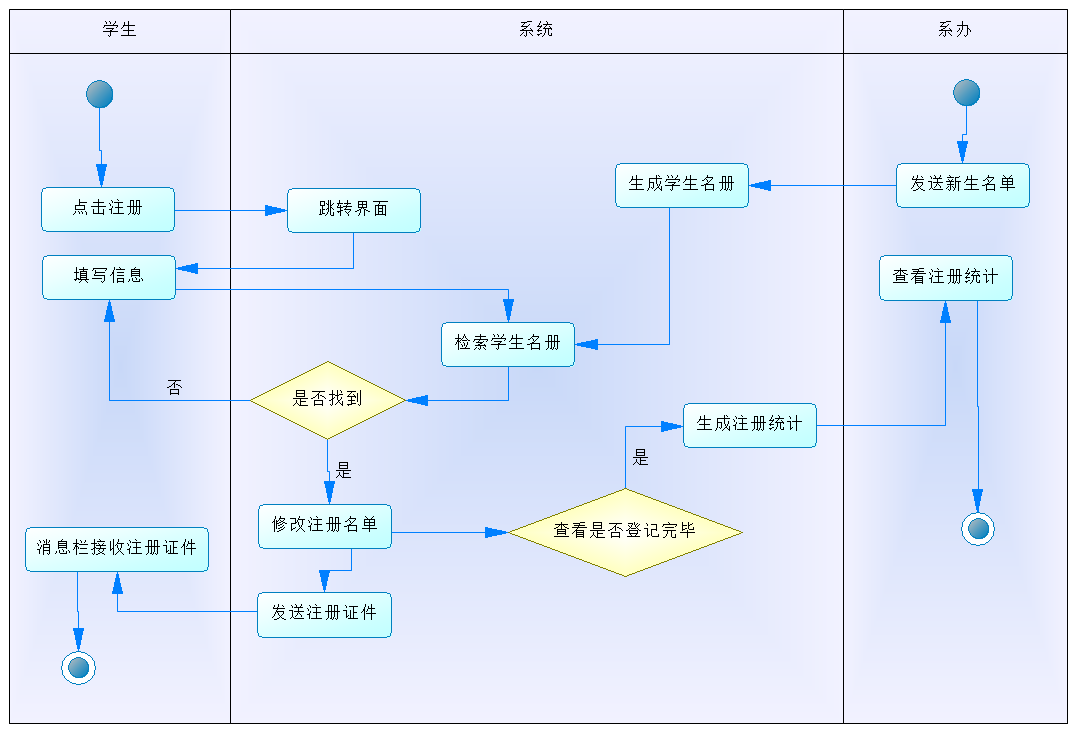
\includegraphics[width = 1\textwidth]{../pic/3/3.1.png}
    \caption{注册活动图}
\end{figure}

\begin{figure}[H]
    \begin{subfigure}{0.5\linewidth}
        \centering
        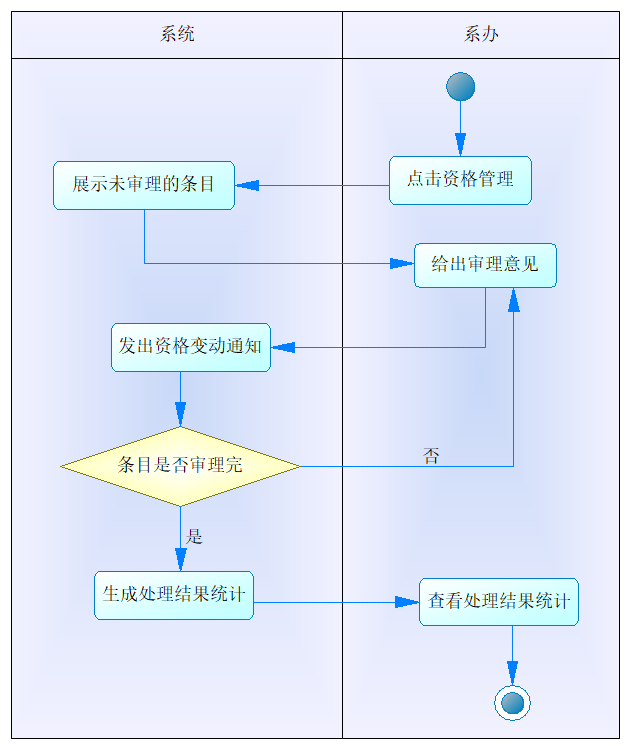
\includegraphics[width = 1\textwidth]{../pic/3/3.2.png}
        \caption{资格管理活动图}
    \end{subfigure}
    \begin{subfigure}{0.5\linewidth}
        \centering
        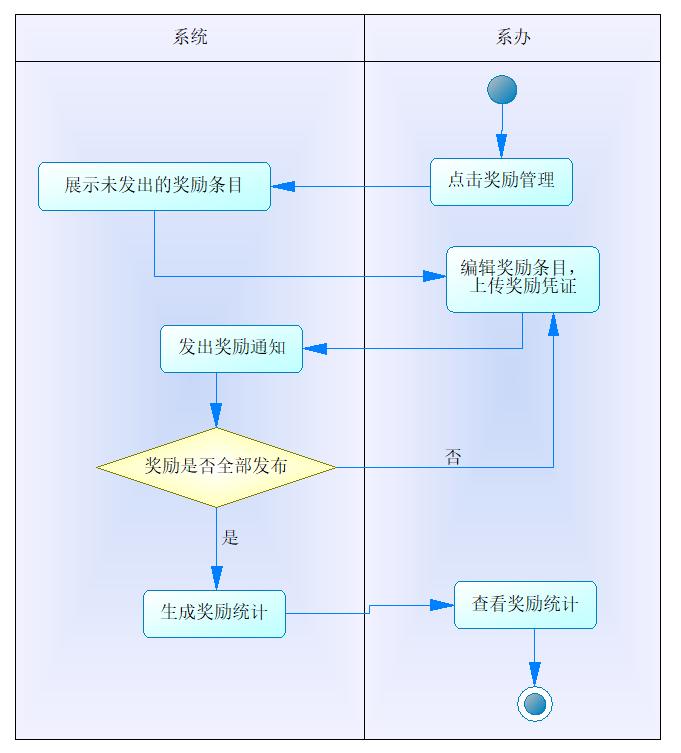
\includegraphics[width = 1\textwidth]{../pic/3/3.3.png}
        \caption{奖励管理活动图}
    \end{subfigure}
\end{figure}

\begin{figure}[H]
    \centering
    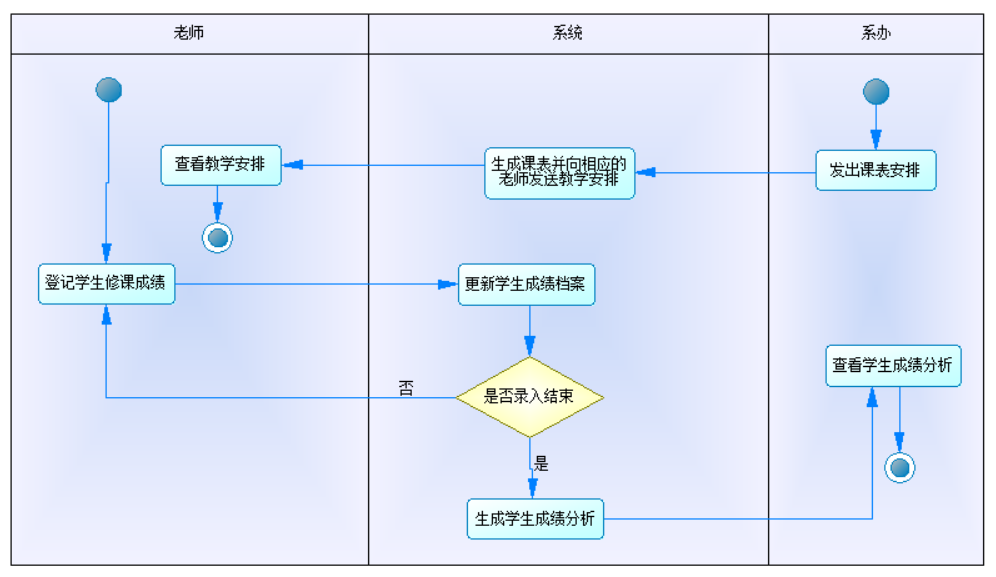
\includegraphics[width = 1\textwidth]{../pic/3/3.4.png}
    \caption{成绩管理活动图}
\end{figure}

\subsection{系统时序图}

分析用例图和用例描述表中的对象关系,结合已有的活动图中体现的事件流,可以得到顺序图。

\begin{figure}[H]
    \centering
    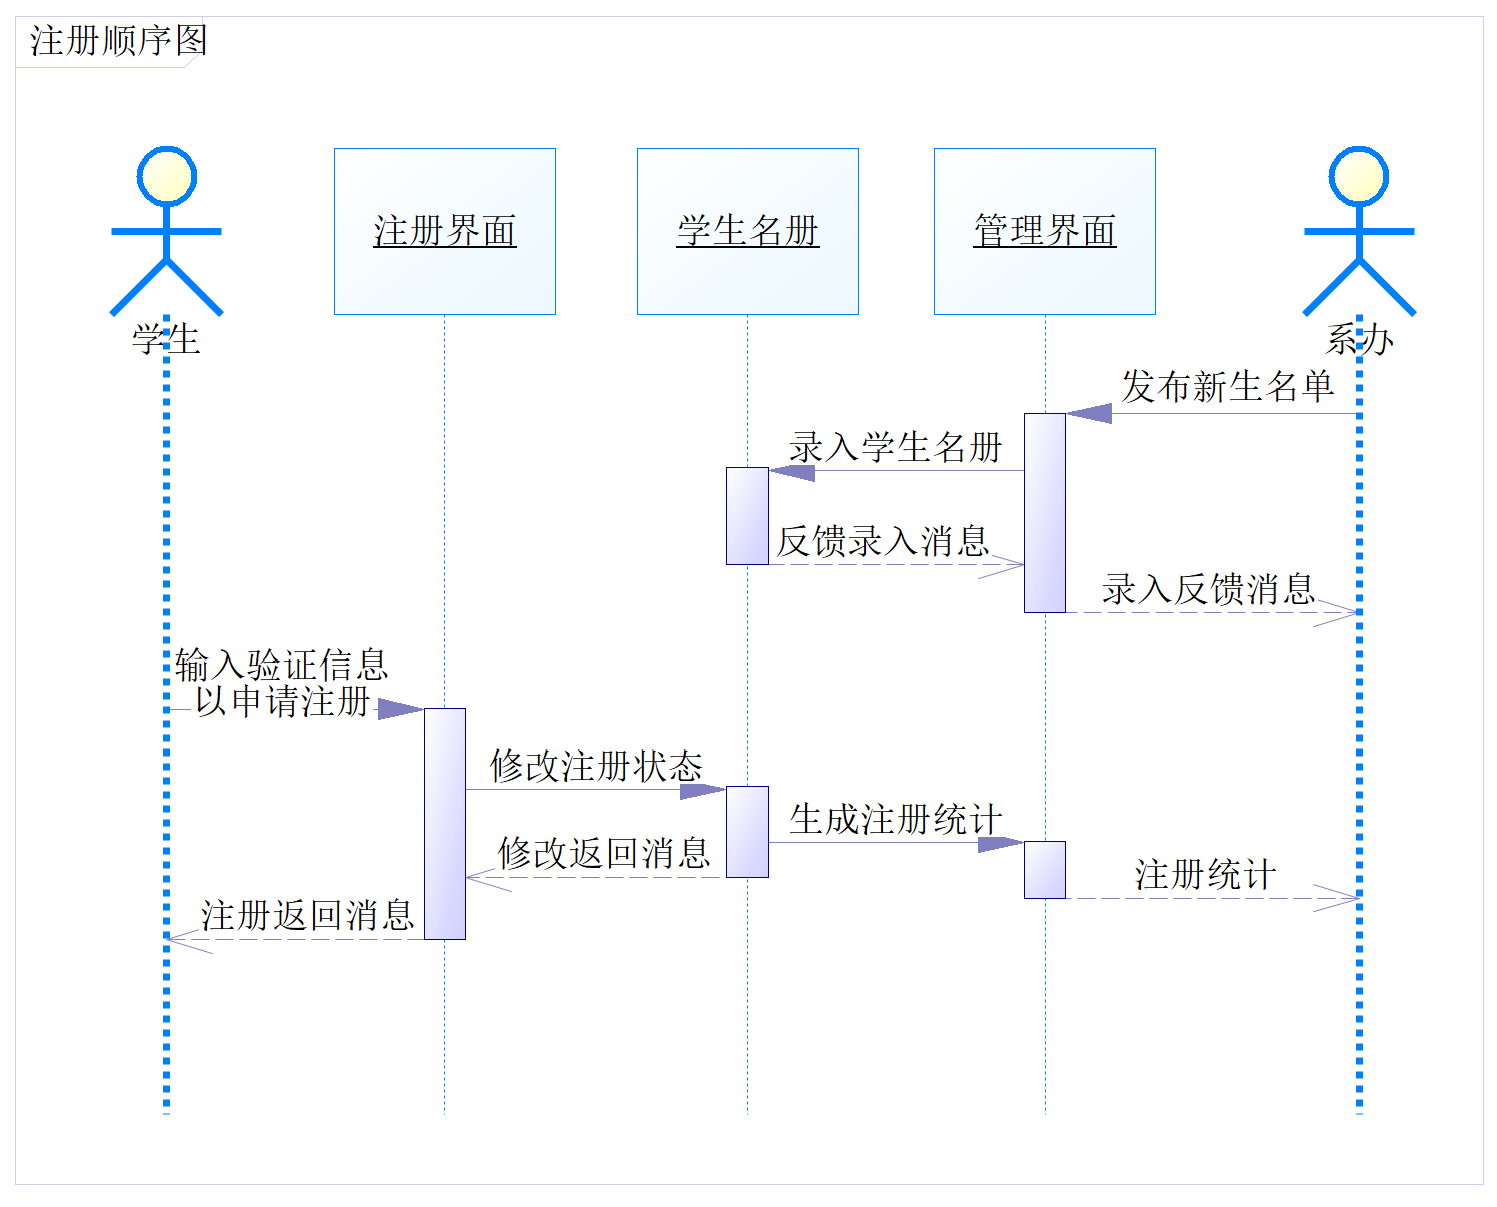
\includegraphics[width = 0.8\textwidth]{../pic/3/3.5.png}
    \caption{注册时序图}
\end{figure}

\begin{figure}[H]
    \centering
    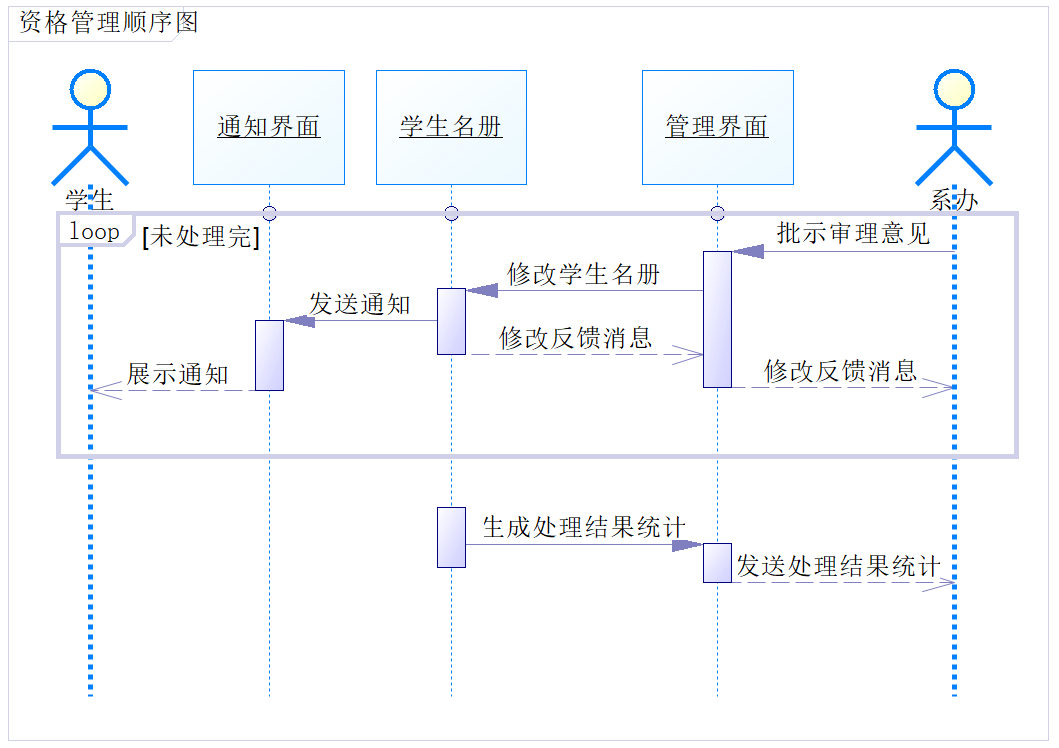
\includegraphics[width = 0.8\textwidth]{../pic/3/3.6.png}
    \caption{资格管理时序图}
\end{figure}

\begin{figure}[H]
    \centering
    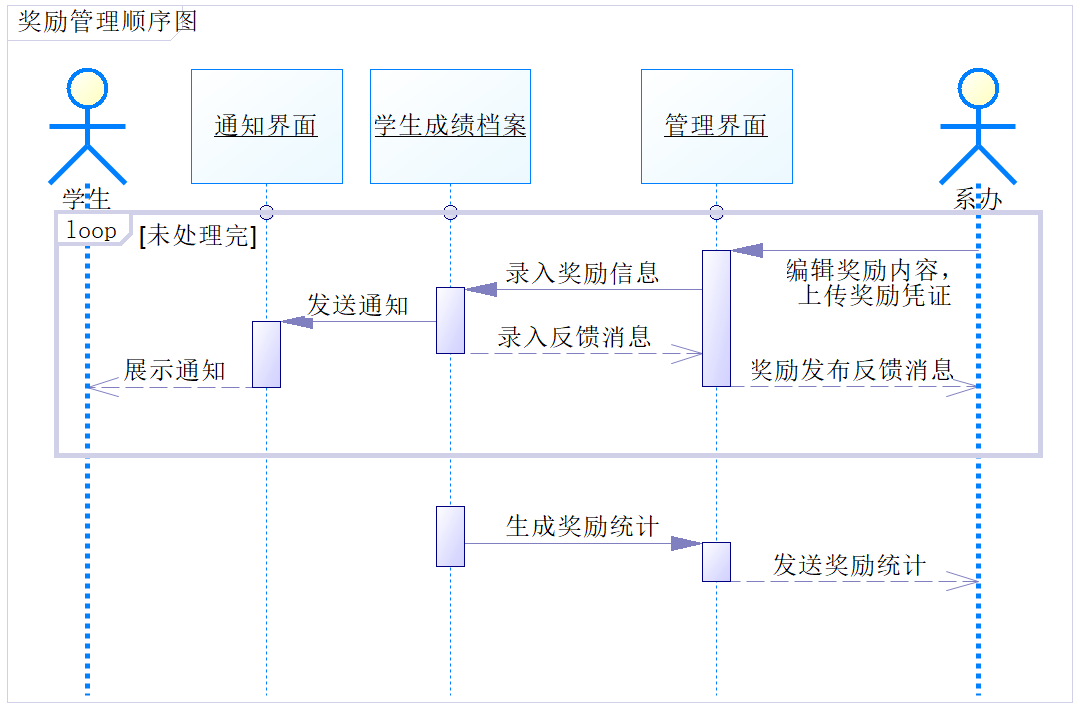
\includegraphics[width = 0.8\textwidth]{../pic/3/3.7.png}
    \caption{奖励管理时序图}
\end{figure}

\begin{figure}[H]
    \centering
    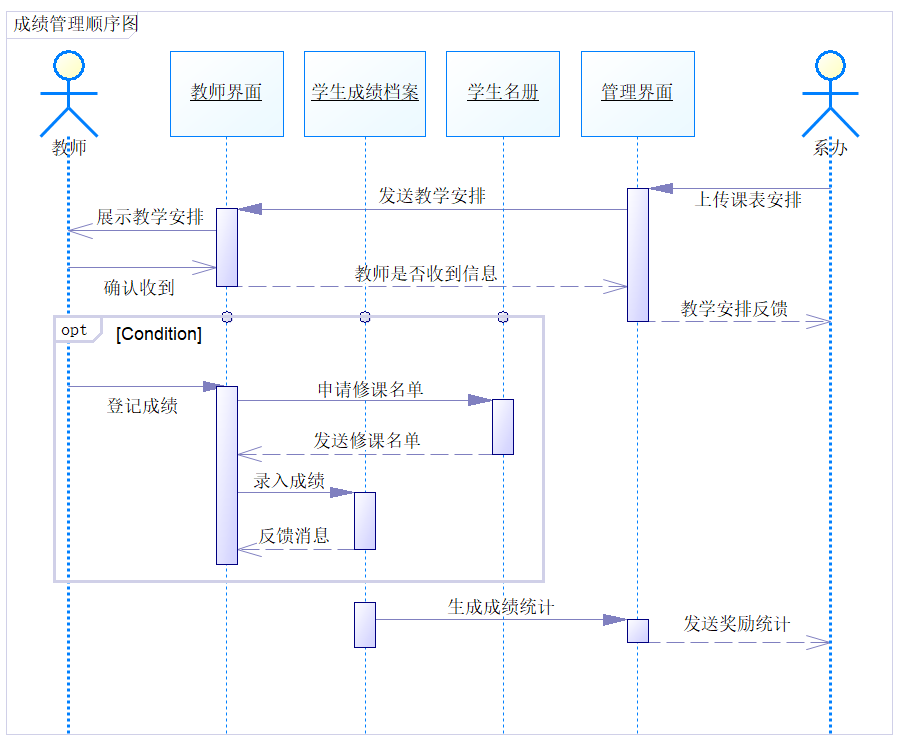
\includegraphics[width = 0.8\textwidth]{../pic/3/3.8.png}
    \caption{成绩管理时序图}
\end{figure}

\section{静态模型(类图)}

\begin{figure}[H]
    \centering
    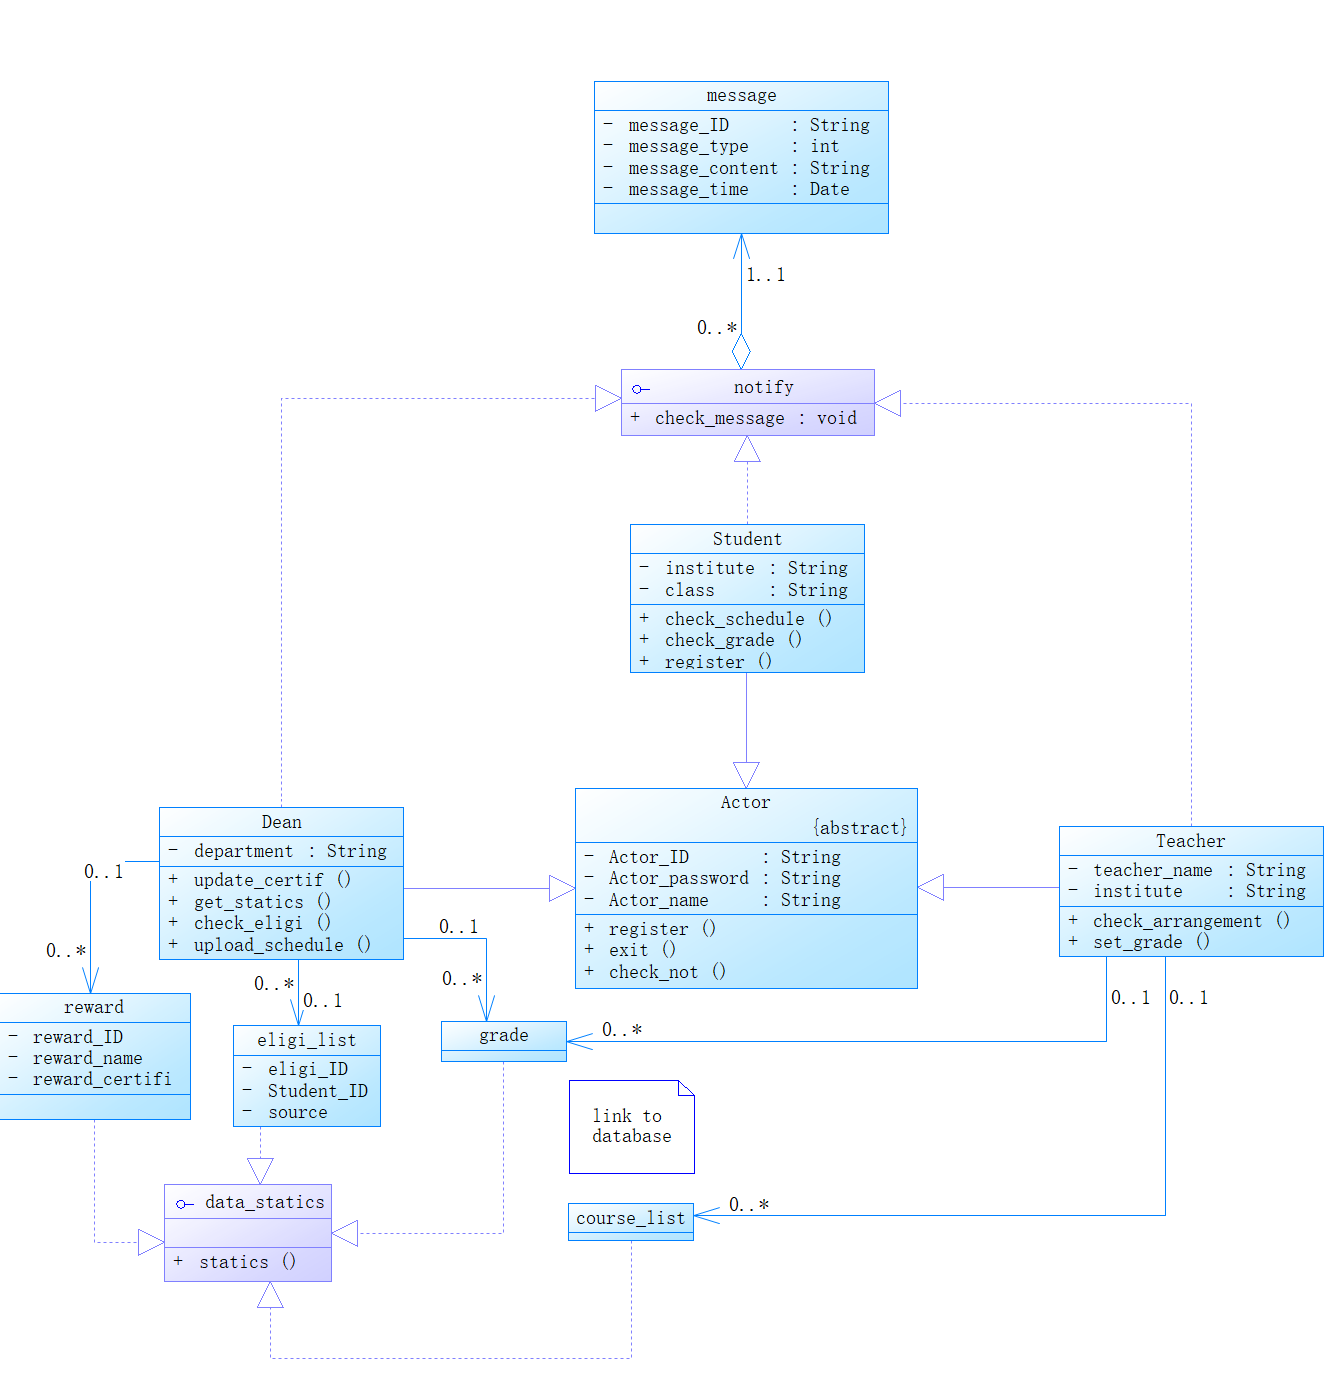
\includegraphics[width = 1\textwidth]{../pic/4/4.1.png}
\end{figure}

\section{ER图}

\begin{figure}[H]
    \centering
    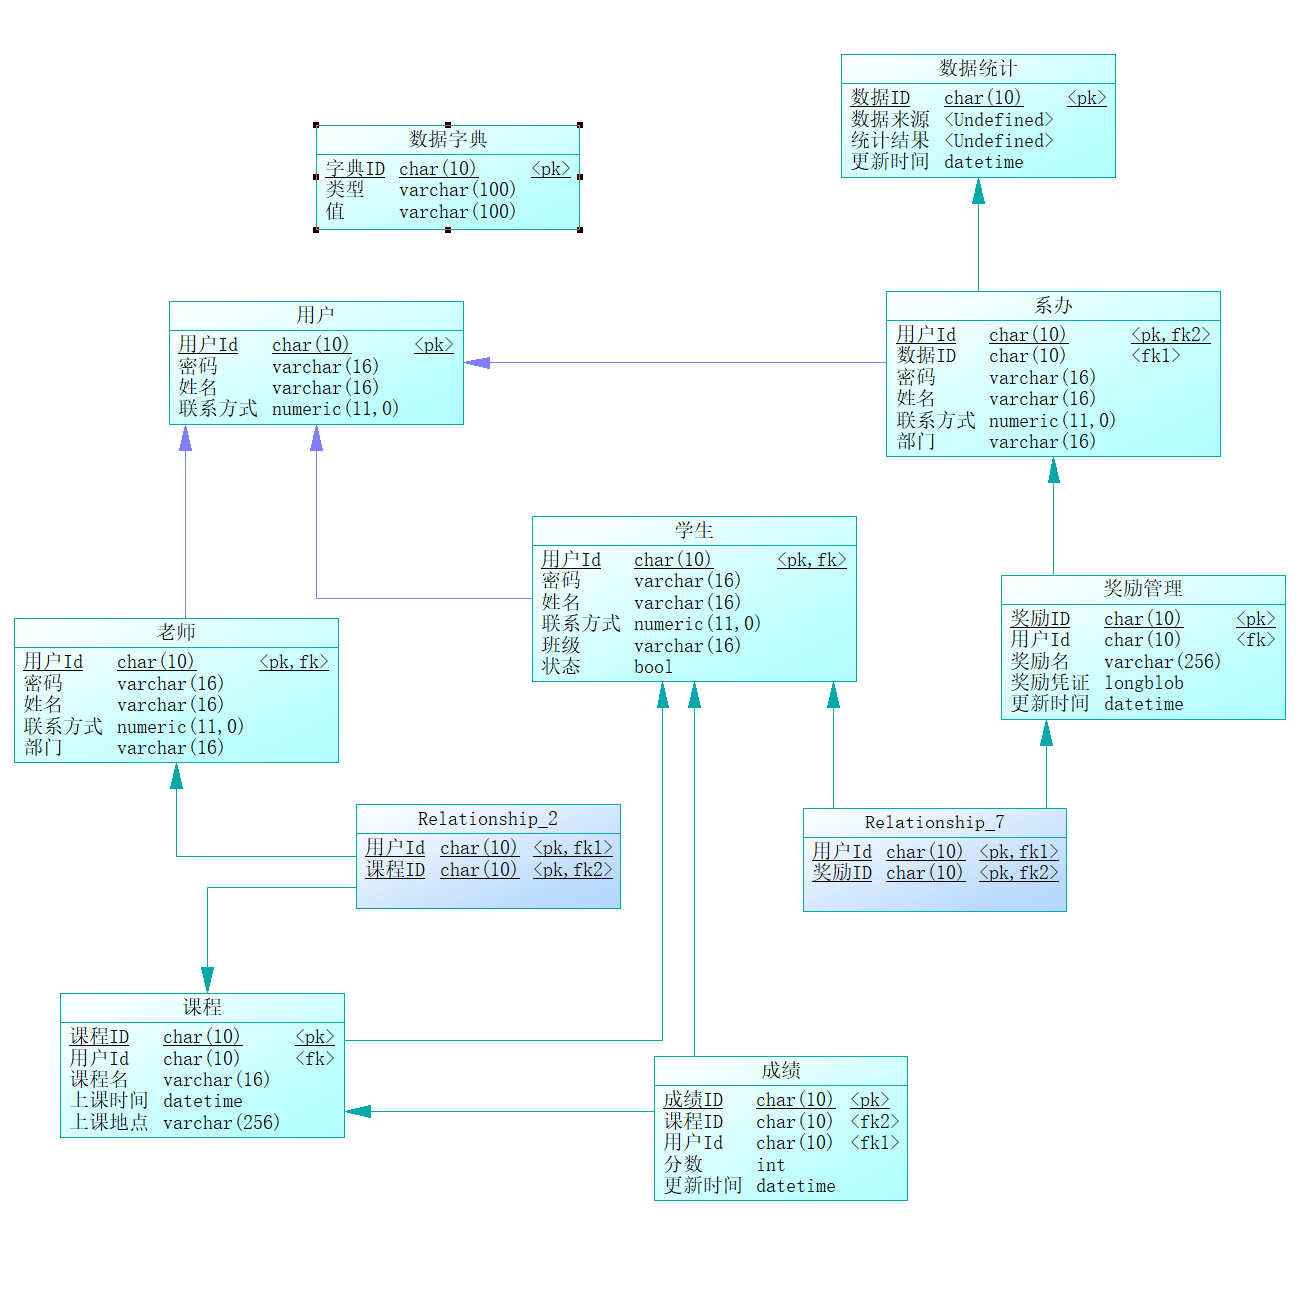
\includegraphics[width = 1\textwidth]{../pic/5/5.1.png}
\end{figure}

\end{document}